\documentclass[conference]{IEEEtran}

% -
% KeySpark project paper.
%
% Compile:  latexmk -pdf main.tex      (or upload this folder to Overleaf,
%           which ships IEEEtran.cls and all packages used below).
%
% Items still to fill before submission are tagged  % TODO(data-freeze)
% (final dataset size + liveness metrics) and  % TODO(figure)  (screenshots).
% Verify EVERY reference in references.bib against the real paper.
% -

\usepackage{cite}
\usepackage{amsmath,amssymb}
\usepackage{graphicx}
\usepackage{booktabs}
\usepackage{tikz}
\usetikzlibrary{positioning,arrows.meta,fit}
\usepackage{xcolor}
\usepackage[hidelinks]{hyperref}
\usepackage{url}

\begin{document}

\documentclass[conference]{IEEEtran}

% -
% KeySpark project paper.
%
% Compile:  latexmk -pdf main.tex      (or upload this folder to Overleaf,
%           which ships IEEEtran.cls and all packages used below).
%
% Items still to fill before submission are tagged  % TODO(data-freeze)
% (final dataset size + liveness metrics) and  % TODO(figure)  (screenshots).
% Verify EVERY reference in references.bib against the real paper.
% -

\usepackage{cite}
\usepackage{amsmath,amssymb}
\usepackage{graphicx}
\usepackage{booktabs}
\usepackage{tikz}
\usetikzlibrary{positioning,arrows.meta,fit}
\usepackage{xcolor}
\usepackage[hidelinks]{hyperref}
\usepackage{url}

\begin{document}

\title{KeySpark: A Real-Time Stream-Processing Pipeline for\\
Keyboard and Mouse Events with Input-Automation Detection}

\author{\IEEEauthorblockN{Murat Emirhan Aykut}
\IEEEauthorblockA{Bah\c{c}e\c{s}ehir University\\
Istanbul, T\"urkiye}}
% TODO(optional): add a contact / student email above if your professor wants one.

\maketitle

\begin{abstract}
Continuous human-computer interaction produces a high-rate, unbounded
stream of keyboard and mouse events that is a natural fit for modern
big-data stream-processing techniques. We present \emph{KeySpark}, an
end-to-end pipeline that captures input events on a host machine, ships
them through a distributed commit log (Apache Kafka), and analyzes them
with Apache Spark using a Lambda architecture: a Structured Streaming
\emph{speed layer} computes low-latency per-minute activity metrics over
event-time tumbling windows, while a periodic Spark \emph{batch layer}
computes order-dependent and session-level analytics (session
segmentation, per-user baselines, spatial heatmaps, and per-day metrics).
As an application of the same content-free signal, a supervised model
classifies each one-minute window as a real person or input automation -
a mouse jiggler, auto-clicker, or keep-awake tool - from cross-modal shape
features, and the dashboard surfaces a flagged day in red. On a single
workstation the pipeline sustains a Structured Streaming throughput of
roughly $2.0\times10^{5}$ rows/s at a mean micro-batch latency of
$275$\,ms, and a batch analytical throughput of roughly
$7.0\times10^{5}$ events/s, over an archive of
% TODO(data-freeze): final event count and collection span.
$\approx\!1.0\times10^{6}$ events collected over twelve days from one
user. On a stratified hold-out the liveness classifier reaches an accuracy
of
% TODO(data-freeze): final accuracy/precision/recall/F1/ROC-AUC from `ml evaluate`.
$\approx\!0.99$; because its non-human class is \emph{synthetic}, we report
this honestly and name validation on real captured automation as future
work. We discuss the engineering trade-offs of the speed/batch split,
exactly-once delivery, and robustness to host sleep/wake.
\end{abstract}

\begin{IEEEkeywords}
stream processing, Apache Spark, Apache Kafka, structured streaming,
Lambda architecture, behavioral analytics, keyboard and mouse dynamics,
input-automation detection, liveness, bot detection.
\end{IEEEkeywords}

% ===========================================================================
\section{Introduction}
\label{sec:intro}
% - Problem Definition (rubric section 1) -

Knowledge work generates a continuous stream of low-level input events:
every key press, mouse movement, click, and scroll. Treated as data, this
is an \emph{unbounded, high-rate event stream}, exactly the regime that
big-data streaming systems are built for. Analyzing it in real time - to
surface live activity metrics and to flag input automation while
preserving privacy - is both a useful application and a representative
systems-engineering problem.

\textbf{Problem.} We address how to capture, transport, and analyze a
continuous stream of keyboard and mouse events such that (i) simple
per-minute activity metrics are available to a live dashboard at low
latency, (ii) richer, order-dependent and session-level analytics are
computed correctly, and (iii) the system tolerates real-world disruptions
such as the host machine sleeping and waking - all without ever persisting
the raw text the user types. As a concrete application of the resulting
stream, we flag \emph{input automation}: whether a minute of activity was
produced by a real person or by a tool such as a mouse jiggler,
auto-clicker, or keep-awake utility.

\textbf{Motivation.} Keystroke and mouse dynamics are an inexpensive,
content-free behavioral signal with established uses in authentication and
behavioral biometrics~\cite{monrose2000keystroke}, and the same
content-free timing and movement signal distinguishes human input from
automated input~\cite{gianvecchio2009botcraft,acien2022becaptcha}. Beyond
the application, the data shape is a canonical big-data challenge: an
unbounded input that must be windowed on \emph{event time}, aggregated
incrementally, made fault-tolerant against producer/consumer rate
mismatch, and split between work that streaming can do cheaply and work
that fundamentally requires a bounded, fully ordered view.

\textbf{Objectives.} KeySpark is designed to:
\begin{itemize}
  \item ingest high-rate input events through a durable, replayable log
        that decouples capture from analysis (Apache Kafka);
  \item compute low-latency per-minute metrics with Spark Structured
        Streaming using event-time tumbling windows, watermarking, and
        an exactly-once columnar sink;
  \item compute order-dependent and session-scoped analytics in a Spark
        batch layer (the Lambda-architecture batch/serving side);
  \item classify each one-minute window as human or input automation (a
        \emph{liveness} signal) from cross-modal shape features, and
        report it honestly;
  \item serve all results to a live web dashboard; and
  \item remain robust to host sleep/wake, while persisting no raw
        keystroke content.
\end{itemize}

\textbf{Contributions.} (1) A complete, reproducible streaming-analytics
pipeline built from standard big-data components. (2) A concrete
justification for the Lambda speed/batch split, driven by metrics whose
correctness requires cross-batch ordering. (3) An honest empirical
evaluation reporting throughput, micro-batch latency, end-to-end latency,
and a per-window human-vs-automation liveness classifier whose non-human
class is synthetic by construction.

% ===========================================================================
\section{Related Work}
\label{sec:related}

\textbf{Stream-processing foundations.} Apache Kafka introduced the
partitioned, replayable commit log as the substrate for decoupling event
producers from consumers~\cite{kreps2011kafka}; it is KeySpark's
ingestion bus. Apache Spark's resilient distributed
datasets~\cite{zaharia2012rdd} provide the fault-tolerant in-memory
engine, and its Structured Streaming API~\cite{armbrust2018structured}
models an unbounded stream as a continuously growing table so that the
same relational operators serve both batch and streaming - the model
KeySpark's speed layer uses directly. The Lambda
architecture~\cite{marz2015bigdata} pairs a low-latency speed layer with
a batch layer that acts as the source of truth; KeySpark is a
concrete, single-machine instantiation of this pattern, with the split
driven by metrics whose correctness requires cross-batch ordering
(Section~\ref{sec:batch}).

\textbf{Streaming systems over interaction data.} The closest
systems-level peers analyze continuous streams of user-interaction
events. Pal et al.~\cite{pal2023clickstream} build a Kafka-based streaming
pipeline over a high-velocity browser clickstream - a close structural
analogue of KeySpark's ingestion, though over web clicks (via Apache Storm
and Markov chains) and aimed at next-click prediction rather than the
per-window classification KeySpark performs over keyboard and mouse
events. Demirezen and Navruz~\cite{demirezen2023lambda} apply the same
Kafka-plus-Spark Lambda stack in an unrelated domain, evidence of the
pattern's generality. Personal-productivity self-monitoring tools such as
TimeAware~\cite{kim2016timeaware} share the interaction-based,
per-time-bin measurement paradigm - its five-minute bins parallel
KeySpark's per-minute windows - but ingest periodically and track
application-usage time rather than streaming raw input events.
KeySpark's niche is thus a true streaming pipeline that computes live
metrics over raw keyboard and mouse events.

\textbf{Keystroke and mouse dynamics as a behavioral signal.} Keystroke
dynamics - content-free timing features such as key hold and flight times
- are an established behavioral biometric for authentication and
identification~\cite{monrose2000keystroke,killourhy2009comparing,teh2013survey}.
The same content-free signal is informative about user state: Epp et
al.~\cite{epp2011identifying} classify a user's emotional state from
keystroke timing, and Acien et al.~\cite{acien2022fatigue} detect mental
fatigue from keystroke dynamics with a deep network. KeySpark reuses these
content-free timing and movement features, but for neither identity nor
affect: it asks whether a minute of input was produced by a human at all,
and never persists the typed text.

\textbf{Detecting input automation.} Distinguishing human from automated
input is a long-standing security problem. Gianvecchio et
al.~\cite{gianvecchio2009botcraft} detect game bots passively, from human
observational proofs in the input stream rather than an interactive
challenge - the same posture KeySpark takes by scoring observed events.
Chu et al.~\cite{chu2012cyborg} classify accounts as human, bot, or cyborg
from behavioral regularity at scale. Closest to our setting, Acien et
al.~\cite{acien2022becaptcha} separate human from bot \emph{mouse}
trajectories and, notably, train partly on \emph{synthetically generated}
trajectories - the same device KeySpark uses for its non-human class, and
the same honesty caveat it carries. KeySpark's niche is a per-window
human-vs-automation liveness signal computed live over a combined keyboard
and mouse stream, content-free, with a synthetic non-human training class
grounded in how real keep-active tools behave.

% ===========================================================================
\section{Dataset Description and Visualization}
\label{sec:dataset}
% - rubric section 3 --

\textbf{Source and collection.} The dataset is self-collected: a native
capture agent records the host's keyboard and mouse events during normal
use. Each event is emitted as a JSON record carrying the event
\texttt{type}, a coarse key identifier or pointer coordinates, the user
id, and an event timestamp \texttt{ts}.
% TODO(data-freeze): final number of events and the collection window.
At the time of writing the archive holds $\approx\!1.0\times10^{6}$
events spanning twelve days from a single user.

\textbf{Privacy by construction.} The agent stores a stable key
\emph{identifier} (the character for printable keys, a symbolic name for
special keys) for timing and counting only; \textbf{no raw typed text is
ever persisted}. Mouse-move events are throttled to roughly $50$/s to
bound volume; clicks and scrolls are never throttled.

\textbf{Format and schema.} Events are parsed into a typed schema
(\texttt{type, key, x, y, button, pressed, dx, dy, user, ts}) and stored
as columnar Parquet, the de-facto analytics format.

\textbf{Features / derived signals.} From the raw events the pipeline
derives, per one-minute window, four counts - keystrokes, words (space
presses), corrections (backspace/delete), and clicks - plus per-user means
and standard deviations of those counts (a baseline). For the liveness
application it additionally derives, per one-minute window, a set of
cross-modal \emph{shape} features that capture the regularity and variety
of input rather than its volume (Section~\ref{sec:ml}).

\textbf{Pre-processing.} Parsing applies an explicit schema (avoiding
costly inference); a watermark bounds late/out-of-order events; mouse
moves are throttled at capture; and idle windows are handled with
divide-by-zero guards in derived ratios.
% TODO(figure): dataset visualization - e.g., histogram of keystrokes
% per window and/or the dashboard's per-minute time series.

% ===========================================================================
\section{Proposed Solution and System Architecture}
\label{sec:arch}
% - rubric section 4 (the core systems contribution) --

\begin{figure*}[t]
\centering
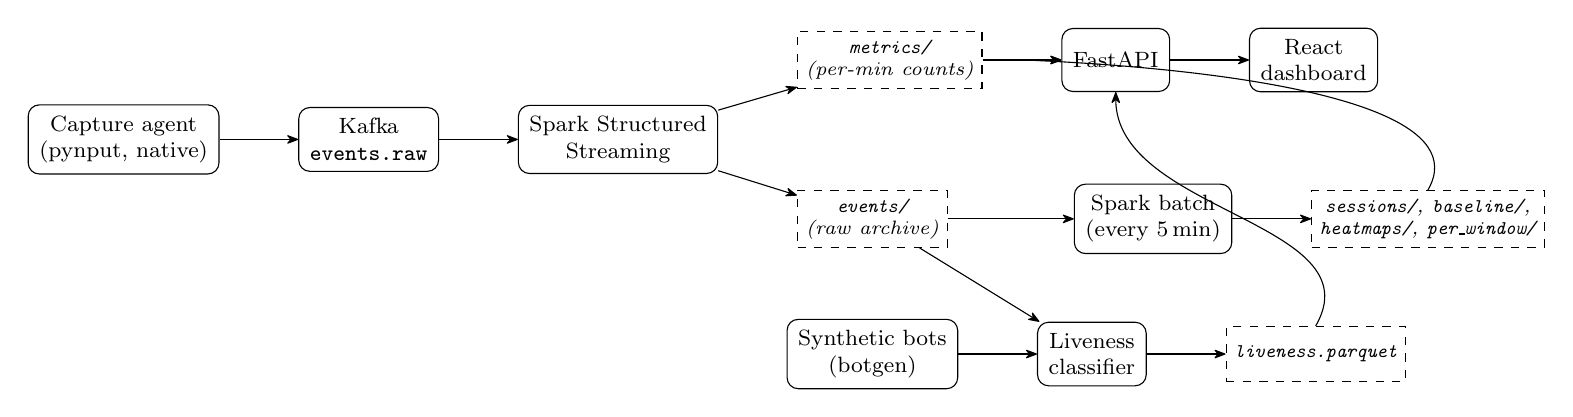
\begin{tikzpicture}[
  >={Stealth[round]},
  box/.style={draw, rounded corners, align=center, font=\footnotesize,
              minimum height=8mm, inner sep=4pt},
  store/.style={draw, dashed, align=center, font=\scriptsize\itshape,
                minimum height=7mm, inner sep=3pt},
  node distance=7mm and 10mm
]
  \node[box] (agent) {Capture agent\\(pynput, native)};
  \node[box, right=of agent] (kafka) {Kafka\\\texttt{events.raw}};
  \node[box, right=of kafka] (stream) {Spark Structured\\Streaming};
  \node[store, above right=2mm and 10mm of stream] (metrics) {\texttt{metrics/}\\(per-min counts)};
  \node[store, below right=2mm and 10mm of stream] (events) {\texttt{events/}\\(raw archive)};
  \node[box, right=16mm of events] (batch) {Spark batch\\(every 5\,min)};
  \node[store, right=of batch] (analytics) {\texttt{sessions/}, \texttt{baseline/},\\\texttt{heatmaps/}, \texttt{per\_window/}};
  \node[box, below=9mm of events] (bots) {Synthetic bots\\(botgen)};
  \node[box, right=of bots] (ml) {Liveness\\classifier};
  \node[store, right=of ml] (liveness) {\texttt{liveness.parquet}};
  \node[box, right=of metrics] (api) {FastAPI};
  \node[box, right=of api] (dash) {React\\dashboard};

  \draw[->] (agent) -- (kafka);
  \draw[->] (kafka) -- (stream);
  \draw[->] (stream) -- (metrics);
  \draw[->] (stream) -- (events);
  \draw[->] (events) -- (batch);
  \draw[->] (batch) -- (analytics);
  \draw[->] (events) -- (ml);
  \draw[->] (bots) -- (ml);
  \draw[->] (ml) -- (liveness);
  \draw[->] (metrics) -- (api);
  \draw[->] (analytics.north) to[out=60,in=180] (api.west);
  \draw[->] (liveness.north) to[out=60,in=-90] (api.south);
  \draw[->] (api) -- (dash);
\end{tikzpicture}
\caption{KeySpark data flow. The agent produces JSON events to Kafka;
Spark Structured Streaming writes per-minute metrics and a raw event
archive; a Spark batch job derives session, baseline, heatmap, and per-day
analytics; a liveness classifier scores the raw event archive (with a
synthetic non-human class from \texttt{botgen}) into
\texttt{liveness.parquet}; and FastAPI serves the Parquet outputs to the
dashboard.}
\label{fig:arch}
\end{figure*}

Figure~\ref{fig:arch} shows the pipeline: capture, ingestion, stream
processing, batch processing, a liveness-scoring branch, and serving. We
describe each in turn and justify the key design decisions.

\subsection{Capture agent}
The agent runs as a native host process because the operating-system
input event tap is not reachable from inside a container. It emits one
JSON event per input action to either standard output (for verification)
or Kafka. It is resilient to host sleep/wake: on wake it re-establishes
the event listeners, and a watchdog detects a silently dead listener and
exits so a supervisor restarts a clean process.

\subsection{Ingestion: Kafka as a replayable log}
The agent does not call Spark directly; it appends each event to the
Kafka topic \texttt{events.raw}, keyed by user~\cite{kreps2011kafka}.
Kafka is a distributed, append-only, partitioned log: it (i) decouples
the producer from the consumer in both time and rate, (ii) persists
events so a consumer can be restarted or replayed without loss, and
(iii) presents the ``unbounded stream'' that Structured Streaming treats
as a growing input table. We run a single broker in KRaft mode, which
removes the former ZooKeeper dependency, in a container.

\subsection{Speed layer: Spark Structured Streaming}
\label{sec:streaming}
Structured Streaming models an unbounded stream as a table that grows by
one row per event, and lets the same relational operators that run on a
static table run incrementally on that growing
input~\cite{armbrust2018structured}. The streaming job consumes
\texttt{events.raw}, casts each Kafka value to a string, and parses it with
an \emph{explicit} schema (avoiding the cost and unpredictability of schema
inference). From this one parsed stream it runs two queries:

\begin{itemize}
  \item \textbf{Query A (metrics).} Events are grouped into one-minute
        \emph{tumbling} windows per user and aggregated into four counts
        (keystrokes, words, corrections, clicks), written once per
        finalized window to \texttt{metrics/}.
  \item \textbf{Query B (archive).} The parsed events are written
        verbatim to \texttt{events/}, the durable, ordered record the
        batch layer and the liveness classifier consume.
\end{itemize}

Sharing one parsed stream means each event is deserialized once and feeds
both sinks. Four streaming concepts are central to correctness:

\textbf{Event time vs.\ processing time.} Windows are defined on the
event's own timestamp, not on when Spark happens to process it. A
``typing minute'' is one minute of real keyboard activity, regardless of
ingestion delay.

\textbf{Watermarking.} Because events can arrive late or out of order, a
watermark (here $5$\,s) tells Spark how long to wait past the largest seen
event time before it considers a window's result final and frees the
window's state. A larger watermark tolerates more lateness at the cost of
holding state, and emitting results, longer.

\textbf{Append output mode.} The Parquet file sink supports only append
mode, which emits each window's row exactly once and never rewrites it.
Append on a windowed aggregation is sound \emph{only} with a watermark:
without one, Spark could never decide that no later event will fall into a
past window, so it could never safely emit that window's row. The
watermark is what makes a windowed aggregation append-compatible.

\textbf{Checkpointing and exactly-once.} Each query checkpoints its Kafka
offsets (and Query~A its window state); combined with the Parquet sink's
atomic, log-based commits, output is end-to-end exactly-once and resumes
cleanly after a restart~\cite{armbrust2018structured}. Each query also runs
on a processing-time trigger ($30$\,s for metrics, $60$\,s for the archive)
that bounds the file-creation rate, and reads with
\texttt{failOnDataLoss=false} so a Kafka log truncated across a host
sleep/wake resets to the earliest available offset rather than crash-looping.

\subsection{Batch layer: order-dependent analytics}
\label{sec:batch}
Some signals cannot be computed correctly on a live stream. Session
boundaries and inter-keystroke timing depend on the \emph{previous} event,
and a \texttt{lag} window function does not see across streaming
micro-batches, so such a computation would silently miss every gap that
straddles a batch boundary. We therefore adopt the Lambda split: the speed
layer lands every event durably and emits the simple counts, and a batch
job over the bounded event archive is the source of truth for
order-dependent and session-level analytics. The batch job runs every five
minutes from an in-process scheduler in the API service. It reads the full
event archive via a file glob (so it processes every recorded event,
independent of the streaming sink's commit log) and computes:

\begin{itemize}
  \item \textbf{Sessions} via the gap-and-island pattern: ordering each
        user's events by event time, flagging a new session whenever the
        idle gap exceeds five minutes, and taking a running cumulative sum
        of those flags as a stable integer session id.
  \item \textbf{Per-user baselines} (mean and standard deviation of each
        per-minute metric), enabling z-score comparison of new activity.
  \item \textbf{Spatial heatmaps} per preset time range, by binning
        pointer coordinates into a fixed grid - spatial windowing
        analogous to time windowing.
  \item \textbf{Per-day metrics}: a per-minute timeline and a spatial
        heatmap keyed by calendar day, which back the dashboard's calendar
        drill-down.
\end{itemize}

\subsection{Liveness model: human vs.\ input automation}
\label{sec:ml}
As an application of the same content-free stream, KeySpark classifies each
one-minute window as a real person or input automation - a \emph{liveness}
signal. The premise is behavioral: human input is irregular and varied,
whereas a jiggler, auto-typer, auto-clicker, or keep-awake tool is regular
and repetitive.

\textbf{Features.} For each one-minute window the model computes seven
\emph{shape} features that are deliberately cross-modal (keyboard and
mouse) and capture regularity and variety rather than volume:
\texttt{key\_diversity} (distinct keys over keystrokes, low for an
auto-typer); the coefficients of variation of the inter-keystroke,
inter-mouse-move, and all-inter-event intervals (\texttt{ks\_iei\_cv},
\texttt{move\_iei\_cv}, \texttt{iei\_cv}; low for a fixed-cadence timer);
the mean and coefficient of variation of the mouse-move step size
(\texttt{step\_mean}, \texttt{step\_cv}; low for a rigid micro-geometry);
and \texttt{mouse\_fraction} (mouse events over all events; near $1$ for a
jiggler, near $0$ for a key-only tool). Windows with fewer than five events
carry no shape evidence and are dropped, so the model abstains on
near-empty minutes rather than guessing.

\textbf{Classes and training.} The human class (label $0$) is the real
event archive; the non-human class (label $1$) is synthetic events from a
generator (Section~\ref{sec:botgen}). Both classes pass through the
\emph{same} featurizer, so there is no train/serve feature skew, and
demo/test bot users are excluded from the human class so a live demo never
poisons the ground truth. We use a random-forest
classifier~\cite{breiman2001random,pedregosa2011scikit} ($300$ trees,
balanced class weights) and evaluate it on a stratified $75/25$ hold-out
(Section~\ref{sec:results}).

\textbf{Real-time use.} After each batch refresh the model scores every
window and aggregates to a per-(user, day) flag: a day is flagged as
automated when at least two of its windows score at least $0.8$, a
sustained burst rather than one odd minute. The flags are written to
\texttt{liveness.parquet} and served to the dashboard, whose calendar
colors a flagged day red.

\subsection{Synthetic non-human class}
\label{sec:botgen}
Because real captured automation is scarce, the non-human training class is
synthetic, generated to match how common keep-active tools actually behave
at the input-event level. A study of verified open-source tools shows that
the only thing such tools randomize is \emph{timing}: their movement
geometry is fixed. Accordingly the generator emits four bot kinds - a mouse
jiggler tracing a fixed relative pattern (diagonal, horizontal, or a small
closed octagon, mirroring the patterns of a widely used open-source
jiggler~\cite{mousejiggler}), a slow keep-awake tool pressing a single
non-character key (an F15-style key, as Caffeine does), an auto-typer over
a small key set, and an auto-clicker - and then jitters their cadence per
session and adds a little cross-modal contamination, so the classifier
cannot separate the classes on the clock or the input mix alone. What
remains for it to learn is the residual robotic tell: a rigid, near-constant
mouse step and a single repeated key. The same featurizer turns these
events into the feature rows above, so synthetic and real data are never
treated differently.

\subsection{Serving layer and deployment}
A small FastAPI service reads the Parquet outputs and serves them as JSON;
a React dashboard polls these endpoints and renders live metric cards, a
per-minute time series, the spatial heatmaps, the session table, and a
history calendar that colors automation-flagged days. We run Spark in
\texttt{local[*]} mode because we process a single user's stream and do not
need a cluster; Kafka runs in a container; only the capture agent must be
native. Each long-running process is wrapped in a restart loop, which
together with Spark checkpointing and the Kafka log gives the pipeline its
baseline sleep/wake resilience. The hard case is a host sleep that leaves
the Spark JVM alive but its local RPC dead, so the streaming job and batch
scheduler keep running yet produce nothing. A watchdog process covers this:
it listens for the operating-system wake notification and bounces the
streaming and API panes after a wake, and otherwise polls output freshness
and probes the Spark RPC, restarting only the wedged component so a single
transient fault does not take the dashboard down.

% ===========================================================================
\section{Results and Discussion}
\label{sec:results}
% - rubric section 5 --

\subsection{Throughput and latency}
We benchmark on the recorded archive on a single workstation
(\texttt{local[*]} Spark). Table~\ref{tab:perf} reports the batch
analytical throughput and the Structured Streaming throughput and
per-micro-batch latency, both measured from Spark's own progress metrics.
% TODO(data-freeze): re-run `python -m keyspark.benchmark batch` and
% `... streaming` on the final archive and update the numbers below.

\begin{table}[t]
\caption{Processing performance on the event archive (single machine).}
\label{tab:perf}
\centering
\begin{tabular}{lrr}
\toprule
Layer & Throughput & Latency \\
\midrule
Spark batch (full pipeline) & $\approx\!7.0\times10^{5}$ ev/s   & - \\ % TODO(data-freeze)
Structured Streaming        & $\approx\!2.0\times10^{5}$ rows/s & $275$\,ms / batch \\ % TODO(data-freeze)
End-to-end (capture$\to$UI) & -                                 & $\approx\!65$\,s \\ % TODO(data-freeze)
\bottomrule
\end{tabular}
\end{table}

The batch layer attains higher per-event throughput because it processes
the archive in a single pass with no per-micro-batch overhead or
watermark-state management; the streaming layer trades some throughput for
incremental, low-latency processing, and its figure is the input row rate
read from Spark's \texttt{StreamingQueryProgress}. The $\approx\!65$\,s
end-to-end latency is dominated \emph{by design} by the one-minute window
plus the watermark, not by engine speed: a per-minute metric cannot be
finalized until its minute has elapsed.

\subsection{Liveness classification}
% TODO(data-freeze): paste the final numbers from `ml evaluate` into the
% table below and update the prose.
Table~\ref{tab:ml} reports accuracy, precision, recall, $F_1$, and ROC-AUC
for the non-human (input automation) class on a stratified hold-out. The
classifier separates the classes almost perfectly, and its most important
features are the all-inter-event and inter-mouse-move interval coefficients
of variation and the mouse-step coefficient of variation - exactly the
timing-and-geometry regularity that distinguishes a tool from a person.

\begin{table}[t]
\caption{Human vs.\ input-automation classification (stratified hold-out).}
\label{tab:ml}
\centering
\begin{tabular}{lr}
\toprule
Metric & Value \\
\midrule
Accuracy  & $0.991$  \\ % TODO(data-freeze)
Precision & $0.976$  \\ % TODO(data-freeze)
Recall    & $0.994$  \\ % TODO(data-freeze)
$F_1$     & $0.985$  \\ % TODO(data-freeze)
ROC-AUC   & $0.9997$ \\ % TODO(data-freeze)
\bottomrule
\end{tabular}
\end{table}

These scores must be read with their main caveat in mind: the non-human
class is \emph{synthetic}, so they partly measure how well the model
separates real data from our own generator rather than from automation in
the wild. We therefore treat the number as evidence that the features are
discriminative, not as a field detection rate. Validation on real captured
automation is future work; usefully, a hardware USB mouse jiggler emits a
genuine HID event stream and so is capturable, unlike the software event
injection that macOS drops.

\subsection{Demonstration}
The live system is demonstrated three ways. Typing updates the per-minute
metrics, time series, and heatmaps on the dashboard within the
window-plus-watermark latency. Injecting a jiggler's events into Kafka
produces a sustained automated burst, and that day's cell on the history
calendar turns red. Throughout, the Spark UI's Structured Streaming tab
shows the input and processing rates in real time.
% TODO(figure): dashboard screenshot (with a flagged day) and Spark UI
% streaming-tab screenshot.

\subsection{Limitations and future work}
The deployment is single-broker, single-user, and single-machine
(\texttt{local[*]}); a multi-user or clustered deployment would exercise
Kafka partitioning and Spark shuffle behavior more fully. The liveness
classifier's strongest limitation is its synthetic non-human class:
training and testing against our own generator inflates the held-out scores
relative to automation in the wild, so validation on real captured
automation - for which a hardware USB jiggler is the natural source, since
its genuine HID events survive capture - is the priority for future work.
Two scope boundaries are inherent to an input-stream detector. Pure
idle-suppressor tools (for example PowerToys Awake~\cite{powertoysawake},
\texttt{caffeinate}, or Amphetamine) keep a machine awake through an
operating-system power assertion and emit no input events at all, so they
are invisible to KeySpark by construction; only input-emitting keep-awake
tools (such as a key-pressing utility) are in range. And a genuine-HID
hardware jiggler that also randomizes its timing is the residual hard case,
detectable, if at all, only by its geometry. The end-to-end latency is
bounded below by the one-minute window; a shorter window would lower it at
the cost of noisier per-minute labels. Host sleep long enough to tear down
Spark's local RPC forces a process restart, so recovery is on the order of
a Spark cold start rather than seconds. Beyond real-bot validation, future
work includes grounding the synthetic generator across the full spectrum of
real keep-active tools, an out-of-stream mode that enumerates power
assertions to catch idle-suppressors, and multi-user or clustered
deployment.

% ===========================================================================
\section{Conclusion}
\label{sec:conclusion}
KeySpark shows that a continuous stream of input events can be captured,
transported, and analyzed end to end with standard big-data components. A
Lambda architecture cleanly separates low-latency per-minute metrics
(Structured Streaming) from order-dependent, session-level analytics
(Spark batch), and, as an application of the same content-free stream, a
random-forest model classifies each minute as human or input automation -
a liveness signal whose non-human class is grounded in verified
keep-active-tool behavior and reported honestly. On a single machine the
pipeline sustains hundreds of thousands of events per second while
preserving user privacy by never storing typed content.

% ===========================================================================
\bibliography{references}
\bibliographystyle{IEEEtran}

\end{document}

\end{document}
